\documentclass[11pt, a4paper]{article}

\usepackage[utf8]{inputenc}
\usepackage[T1]{fontenc}
\usepackage{lmodern}
\usepackage{amsmath, amssymb}
\usepackage{graphicx}
\usepackage{float}
\usepackage{placeins}
\usepackage{booktabs}
\usepackage{multirow}
\usepackage{hyperref}
\usepackage{geometry}
\usepackage{caption}
\usepackage{subcaption}
\usepackage{xcolor}

\geometry{
  a4paper,
  left=25mm,
  right=25mm,
  top=25mm,
  bottom=25mm
}

\hypersetup{
    colorlinks=true,
    linkcolor=blue,
    filecolor=magenta,      
    urlcolor=cyan,
    citecolor=blue,
}

\title{\textbf{Topology-Aware Byzantine Defense in Hierarchical Federated Learning: Comparative Study of Soft Cosine Rejection across Network Topologies and Data Partitioning Strategies}}

\author{
    \textbf{Hung Anh Nguyen} \\
    \small Bachelor of Science in Computer Science, College of Engineering and Computer Science \\
    \small VinUniversity, Hanoi, Vietnam \\
    \small \texttt{25anh.nch@vinuni.edu.vn}
}
\date{\today}


\begin{document}

\maketitle

\begin{abstract}
Federated Learning (FL) under non-IID data distributions is vulnerable to Byzantine attacks such as label flipping. Different network topologies, including Centralized Star (FedAvg, Ditto), Decentralized Ring, and Hierarchical Ensemble (HE), exhibit varying degrees of resilience against adversarial updates. In this work, I investigate combining a \textit{Soft Cosine Rejection Aggregator} (a trust-weighted aggregation mechanism) with the Hierarchical Ensemble (HE) topology, deploying defenses at both the cluster and global aggregation levels. Furthermore, I formulate and employ a \textit{Bilevel Dirichlet Partitioning strategy} with dual concentration parameters ($\alpha_{\text{inter}}, \alpha_{\text{intra}}$) to systematically evaluate realistic data heterogeneity across clusters and clients. Comprehensive experiments on the CIFAR-10 benchmark demonstrate the behavior of each topology under attack. On a standard non-IID partition ($\alpha=0.1$), the HE topology with Full Defense maintains an accuracy of 89.50\% under a 30\% adversarial ratio ($q=0.3$), whereas the undefended HE baseline degrades to 9.95\%. Under the hierarchical partition setting, HE with Full Defense exhibits consistent convergence, maintaining approximately 37--46\% accuracy. These empirical findings demonstrate the utility of topology-aware defense placement for mitigating Byzantine adversaries in hierarchical federated learning.
\end{abstract}

\vspace{0.5cm}

\section{Introduction}

Federated Learning (FL) enables distributed model training across decentralized edge devices without centralizing raw private data \cite{mcmahan2017}. Despite its privacy-preserving advantages, practical FL deployments face two fundamental challenges: \textit{statistical heterogeneity} (non-IID data distributions across clients that induce client drift and hinder model convergence) and \textit{vulnerability to Byzantine adversaries} (compromised nodes submitting poisoned updates, such as label-flipping attacks, to subvert the global model) \cite{blanchard2017, zhao2018}. While various robust aggregation rules have been proposed, the interplay between \textit{network communication topologies} (e.g., centralized star, decentralized ring, and multi-tier hierarchical structures) and Byzantine resilience remains insufficiently characterized. Furthermore, standard benchmarks predominantly simulate non-IID data using a single global concentration parameter, failing to reflect the structured, multi-tier data heterogeneity observed in real-world institutional federations.

To address these limitations, I investigate the Byzantine robustness of the Hierarchical Ensemble (HE) topology integrated with a \textit{Soft Cosine Rejection Aggregator}. By deploying trust-weighted cosine filtering across both cluster-level and global-level aggregation tiers, the system creates a multi-stage defense barrier against malicious gradient updates. Additionally, I formulate a \textit{Bilevel Dirichlet Partitioning strategy} governed by dual concentration parameters ($\alpha_{\text{inter}}, \alpha_{\text{intra}}$) to capture realistic cluster-level specialization and intra-cluster client variance. 

In summary, the primary contributions of my research are as follows:
\begin{itemize}
    \item \textit{Bilevel Dirichlet Partitioning Formulation:} I design and implement a two-level partitioning framework parameterized by ($\alpha_{\text{inter}}, \alpha_{\text{intra}}$) to systematically model structured semantic skew across clusters and edge clients.
    \item \textit{Multi-Tier Soft Cosine Defense:} I develop and implement a Byzantine-resilient aggregator based on directional normalization, adaptive temperature scaling, and norm bounding, deployed across multi-tier hierarchical aggregation scopes.
    \item \textit{Comprehensive Empirical Benchmark:} I conduct an extensive evaluation comprising over 100 experimental runs across 4 topologies, 4 attack fractions ($q \in \{0, 0.1, 0.2, 0.3\}$), and 2 partitioning strategies on the CIFAR-10 benchmark.
    \item \textit{Open-Source Evaluation Suite:} I release the complete codebase, experiment configurations, and reproducible evaluation pipeline at \url{https://github.com/nam200718/Topology-aware-FDL.git}. My individual contributions specifically encompass the Byzantine defense pipeline (\texttt{src/defense/}), multi-topology experimental drivers (\texttt{temp/}), and standardized Jupyter execution notebooks (\texttt{notebook\_training/}).
\end{itemize}

The remainder of this paper is organized as follows: Section 2 reviews related work. Section 3 outlines the system architecture, data partitioning formulation, and defense mechanism. Section 4 describes the experimental setup. Section 5 presents empirical results and discussion. Finally, Section 6 concludes the paper.

\section{Related Work}

\subsection{Federated Learning Fundamentals}
Standard FL formulations such as FedAvg \cite{mcmahan2017} rely on a centralized star architecture for model parameter aggregation. Personalized FL methods, including Ditto \cite{li2021}, introduce local proximal regularization terms to address statistical heterogeneity. The theoretical and empirical challenges associated with non-IID client distributions have been widely analyzed in the literature \cite{zhao2018, karimireddy2020}.

\subsection{Decentralized \& Hierarchical FL}
Decentralized topologies, such as Ring and Gossip communication networks, eliminate the central parameter server by having clients exchange parameters solely with local neighbors. Hierarchical FL \cite{liu2020} introduces multi-tier aggregation via intermediate cluster heads. In this work, the underlying Shared-Backbone Multi-Head model architecture of the Hierarchical Ensemble (HE) was designed collaboratively by teammates, whereas the multi-tier defense integration, bilevel data partitioning strategy, and comprehensive benchmarking suite constitute my independent work.

\subsection{Byzantine-Resilient Aggregation}
Existing Byzantine defenses include distance-based coordinate filtering such as Krum and Multi-Krum \cite{blanchard2017}, robust statistical estimators like Trimmed Mean and Coordinate-wise Median \cite{yin2018}, angular similarity techniques such as FoolsGold \cite{fung2020}, and norm bounding constraints \cite{sun2019}. In this study, my Soft Cosine Rejection aggregator couples directional cosine filtering, softmax temperature scaling, and dynamic norm bounds within multi-tier hierarchical aggregation.

\subsection{Data Partitioning in FL}
The Dirichlet distribution is standard for generating synthetic Non-IID partitions in FL benchmarks \cite{hsu2019}. However, prevailing approaches predominantly apply a single global parameter $\alpha$, which fails to capture multi-tier hierarchical groupings observed in real-world institutional federations (e.g., regional hospital clusters).

\section{Methodology}

\subsection{System Overview}
The simulated environment comprises 30 clients partitioned across 5 clusters evaluated on CIFAR-10. I evaluate four primary communication topologies: Star (FedAvg), Star (Ditto), Ring, and Hierarchical Ensemble (HE). In the HE framework, client updates are first aggregated locally at intermediate cluster heads before intermediate representations are consolidated at the central server.

\subsection{Bilevel Dirichlet Partitioning Strategy}
\textit{Objective:} To simulate realistic federated distributions where data is heterogeneous not only across individual edge clients but also exhibits structured semantic specialization across organizational clusters.

\textit{Formulation and Dual Parameters:} Rather than generating data through an unstructured single-step draw, data distribution is governed by two distinct Dirichlet concentration parameters:
\begin{itemize}
    \item \textit{Inter-Cluster Allocation ($\alpha_{\text{inter}}$, or $\beta$):} Controls class distribution across the $K$ clusters. A smaller value of $\alpha_{\text{inter}}$ induces pronounced specialization, where each cluster predominantly holds a small subset of labels.
    \item \textit{Intra-Cluster Allocation ($\alpha_{\text{intra}}$, or $\chi$):} Controls the distribution of the cluster's allocated samples among the $M/K$ clients assigned to that cluster. A larger $\alpha_{\text{intra}}$ produces a relatively balanced distribution among internal peers, whereas a smaller value introduces secondary non-IID variance within the cluster.
\end{itemize}

In my benchmark experiments, I configure $\alpha_{\text{inter}} = 0.1$ to enforce strong inter-cluster specialization and $\alpha_{\text{intra}} = 1.0$ for moderate intra-cluster client variance.

\begin{figure}[H]
    \centering
    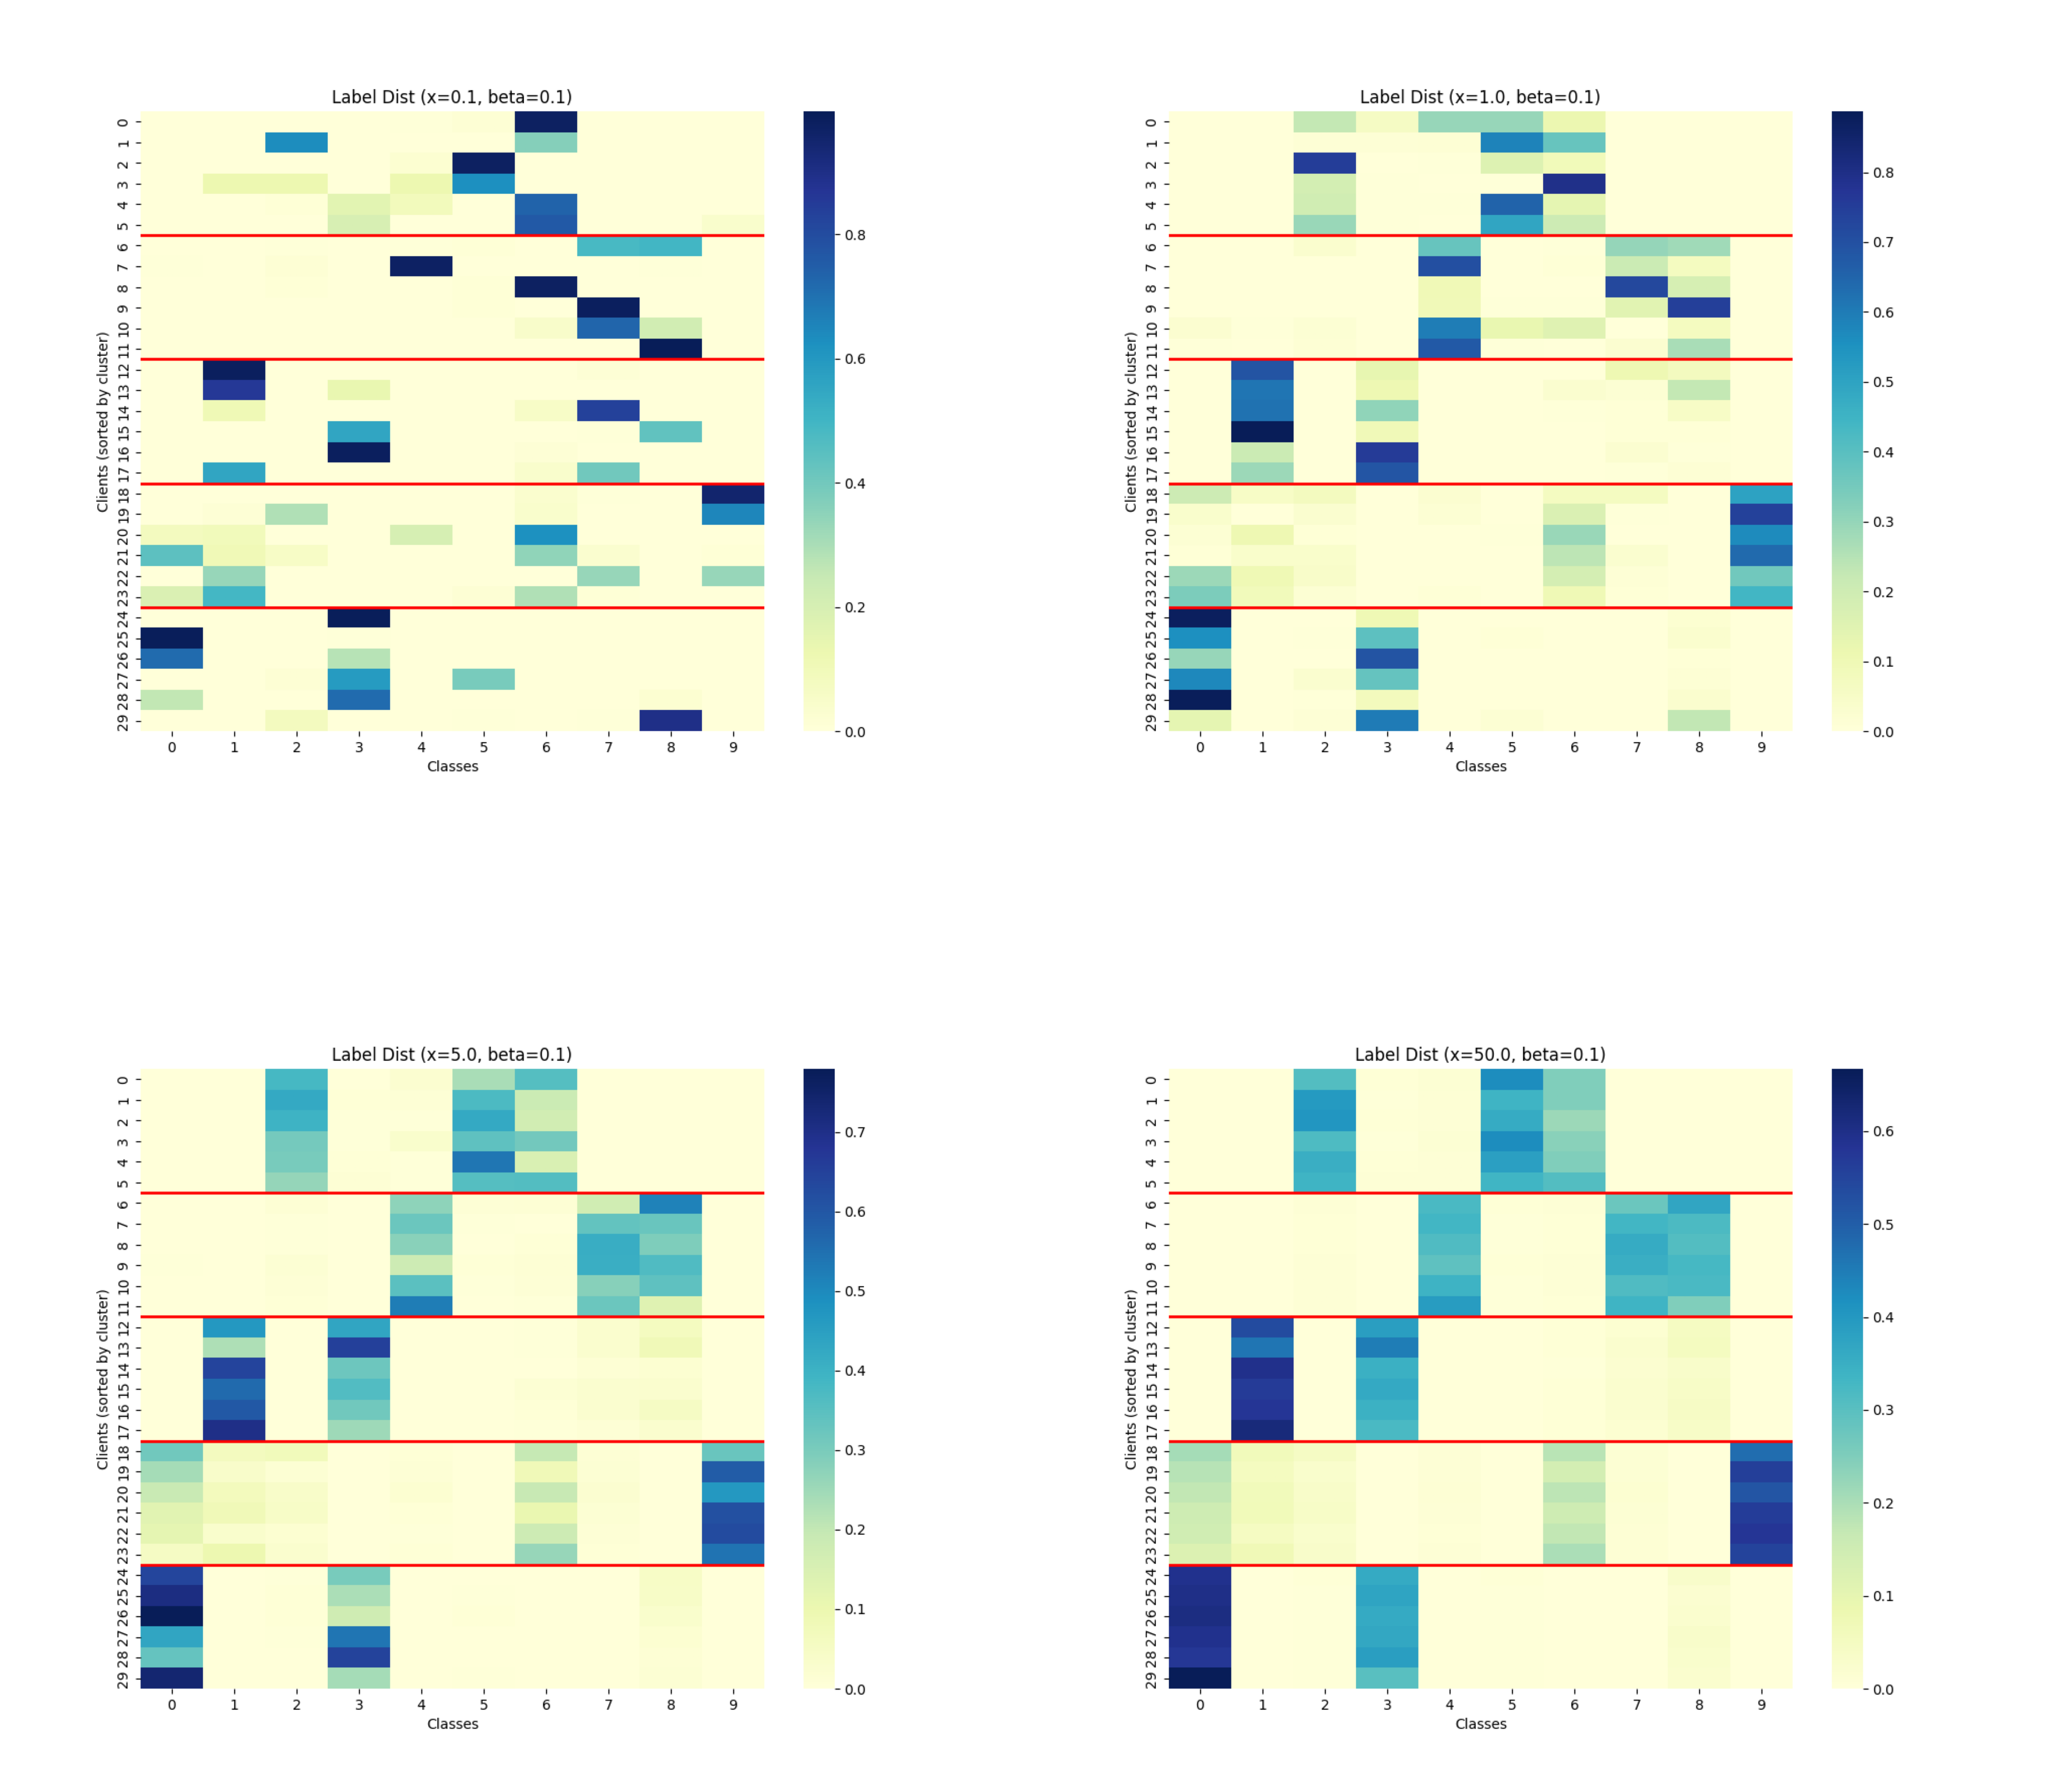
\includegraphics[width=0.9\textwidth]{E1_data_partitioning.png}
    \caption{Class label distributions for 30 clients $\times$ 10 classes across various ($\alpha_{\text{intra}}=\chi, \alpha_{\text{inter}}=\beta$) configurations. Red vertical lines delineate cluster boundaries.}
    \label{fig:partitioning}
\end{figure}

\subsection{Soft Cosine Rejection Aggregator}
The proposed defense mechanism processes client updates through the following sequential operations:
\begin{enumerate}
    \item \textit{Compute Update Delta:} $\Delta w_i = w_i^{\text{after}} - w_{\text{reference}}$
    \item \textit{Directional Normalization:} $\hat{\Delta}_i = \Delta_i / \|\Delta_i\|$ to mitigate magnitude inflation attacks.
    \item \textit{Directional Centroid Calculation:} $\bar{\Delta} = \frac{1}{n}\sum_{i=1}^n \hat{\Delta}_i$
    \item \textit{Cosine Similarity Computation:} $s_i = \cos(\Delta_i, \bar{\Delta}) = \frac{\Delta_i \cdot \bar{\Delta}}{\|\Delta_i\| \cdot \|\bar{\Delta}\|}$
    \item \textit{Dynamic Norm Bounding:} Bound update magnitudes $\|\Delta_i\|$ against a dynamic threshold defined as $\text{median}(\{\|\Delta_j\|\}) \times \gamma$.
    \item \textit{Adaptive Temperature Scaling:} Adjust temperature $\tau$ inversely with respect to sample variance $\mathrm{Var}(s_i)$, tightening trust margins when directional dispersion increases.
    \item \textit{Trust Weight Assignment:} Compute normalized aggregation weights $\alpha_i$ via softmax:
    \begin{equation}
        \alpha_i = \frac{\exp(s_i / \tau)}{\sum_{j=1}^n \exp(s_j / \tau)}
    \end{equation}
    \item \textit{Weighted Parameter Aggregation:} $w_{\text{agg}} = \sum_{i=1}^n \alpha_i \cdot w_i$
\end{enumerate}

A \textit{Sentinel Pre-filter} is executed prior to aggregation to immediately disqualify updates exhibiting numerical instability ($\mathrm{NaN}/\mathrm{Inf}$).

\subsection{Defense Scope: Cluster-Level vs. Global-Level}
\begin{itemize}
    \item \texttt{defense\_scope: cluster}: Defense is applied exclusively during Phase 1 cluster-head aggregation.
    \item \texttt{defense\_scope: global}: Defense is applied exclusively during Phase 2 central server aggregation.
    \item \texttt{defense\_scope: both}: Defense is deployed simultaneously at both aggregation tiers (\textit{Full Defense}).
\end{itemize}
Unlike single-tier architectures (Star, Ring), the HE topology enables hierarchical multi-stage filtering.

\subsection{Byzantine Adversary Model}
I evaluate resilience against a \textit{Label Flipping Attack}, wherein adversarial clients perturb their training labels according to the mapping $y \mapsto (C - 1 - y)$ prior to local optimization. I evaluate adversarial proportions $q \in \{0.0, 0.1, 0.2, 0.3\}$.

\section{Experimental Setup}

\subsection{Dataset \& Model}
\begin{table}[H]
    \centering
    \begin{tabular}{ll}
        \toprule
        \textbf{Parameter} & \textbf{Value} \\
        \midrule
        Dataset & CIFAR-10 (60,000 images, 10 classes) \\
        Model Architecture & ResNet-9 ($\sim$1.65M parameters) \\
        Number of Clients & 30 \\
        Number of Clusters (HE) & 5 \\
        Local Batch Size & 128 \\
        Local Learning Rate & 0.01 \\
        Local Epochs/Steps & 2 \\
        Communication Rounds & 50 \\
        Non-IID Partition Parameter (Random) & Dirichlet $\alpha = 0.1$ \\
        Random Seed & 42 \\
        \bottomrule
    \end{tabular}
    \caption{Summary of experimental hyperparameters.}
\end{table}

\subsection{Experiment Matrix}
A total of 68 experimental runs were executed across 5 core evaluation stages:
\begin{itemize}
    \item \textit{Data Partitioning Analysis:} Validation and heatmap characterization of the bilevel Dirichlet distribution across clusters.
    \item \textit{Baseline Convergence on Random Partition:} Benchmarking 4 topologies under standard Dirichlet non-IID conditions ($\alpha=0.1$) without adversaries.
    \item \textit{Convergence on Bilevel Hierarchical Partition:} Evaluating topology convergence under structured inter-cluster heterogeneity ($\alpha_{\text{intra}}=1.0, \alpha_{\text{inter}}=0.1$).
    \item \textit{Byzantine Robustness on Random Partition:} Assessing defense effectiveness against label flipping ($q \in \{0, 0.1, 0.2, 0.3\}$) on standard non-IID data.
    \item \textit{Byzantine Robustness on Bilevel Hierarchical Partition:} Stress-testing multi-tier defense capabilities under combined label flipping attacks and structured data skew.
\end{itemize}

\subsection{Code Availability and Reproducibility}
All source code, configuration files, and evaluation scripts are publicly available at \url{https://github.com/nam200718/Topology-aware-FDL.git}. Specifically, my individual contributions encompass:
\begin{itemize}
    \item Byzantine defense pipeline implementations and YAML configurations in directory \texttt{src/defense/}.
    \item Multi-topology experiment execution drivers, bilevel data partitioning utilities, and visualization scripts located in directory \texttt{temp/}.
    \item Standardized Jupyter execution notebooks in directory \texttt{notebook\_training/} for reproducing all baseline convergence trajectories and Byzantine attack sweeps.
    \item Report source code, LaTeX templates, and visual artifacts located in directory \texttt{outputs/REPORT/}.
\end{itemize}

\section{Results \& Discussion}

\subsection{Characterization of Bilevel Data Partitioning}
Figure \ref{fig:partitioning} illustrates class allocations across various parameter combinations. The setting $(\alpha_{\text{intra}}=1.0, \alpha_{\text{inter}}=0.1)$ creates clear cluster-level semantic focus while retaining intra-cluster sample diversity. Lower values ($\alpha_{\text{intra}}=0.1$) lead to extreme class sparsity per client, whereas higher values ($\alpha_{\text{intra}}=50.0$) homogenize internal distributions, reducing cluster distinction.

\subsection{Convergence Dynamics on Standard Non-IID Partition}
\begin{figure}[H]
    \centering
    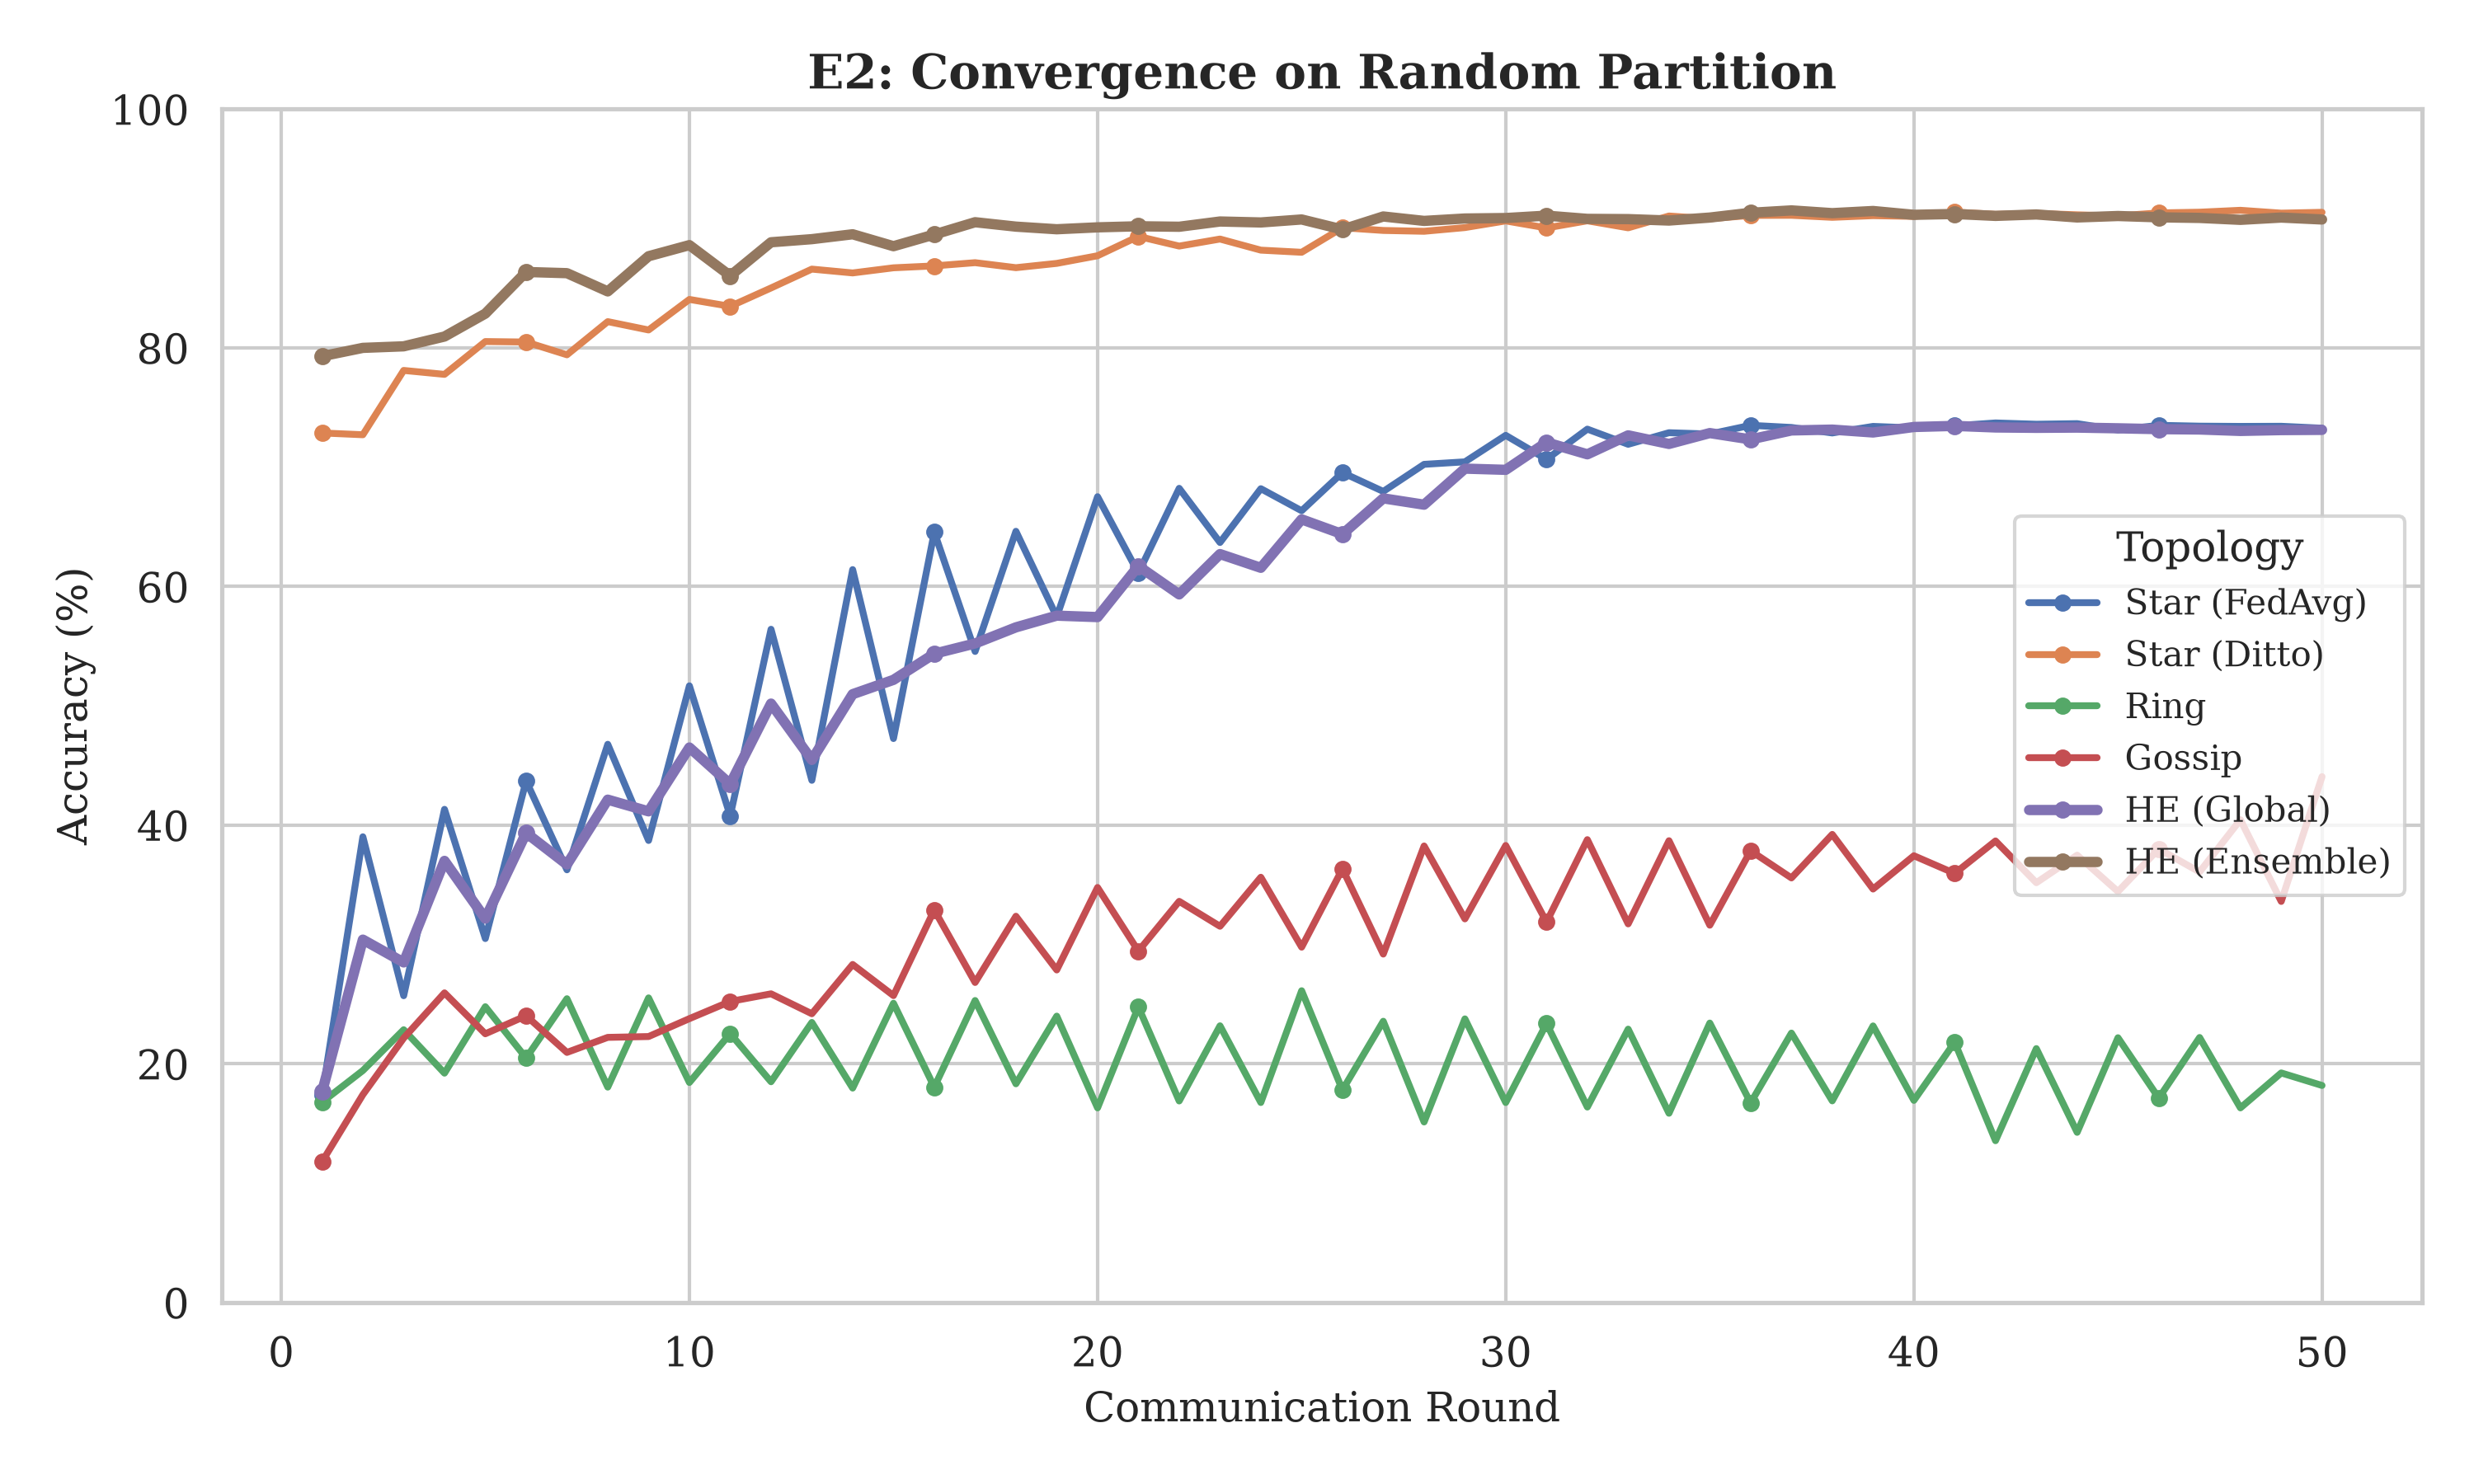
\includegraphics[width=0.75\textwidth]{partA_E2_random_accuracy.png}
    \caption{Convergence trajectories on Random Partition ($\alpha=0.1$) over 50 communication rounds.}
    \label{fig:e2}
\end{figure}

\begin{table}[H]
    \centering
    \begin{tabular}{lc}
        \toprule
        \textbf{Topology} & \textbf{Final Accuracy (\%)} \\
        \midrule
        Star (Ditto) — personalized & 91.35 \\
        HE (Ensemble) — personalized & 90.75 \\
        Star (FedAvg) — global & 73.25 \\
        HE (Global) & 73.12 \\
        Gossip ($k=3$) & 44.06 \\
        Ring & 18.18 \\
        \bottomrule
    \end{tabular}
    \caption{Final Accuracy (Round 50) — Random Partition ($\alpha=0.1$)}
\end{table}

Personalized architectures (Ditto and HE Ensemble) achieve superior accuracy ($\sim$91\%) compared to global parameter averaging ($\sim$73\%) under non-IID conditions. Decentralized baselines without central coordination (Ring, Gossip) exhibit substantially slower convergence rates.

\subsection{Convergence Dynamics on Bilevel Hierarchical Partition}
\begin{figure}[H]
    \centering
    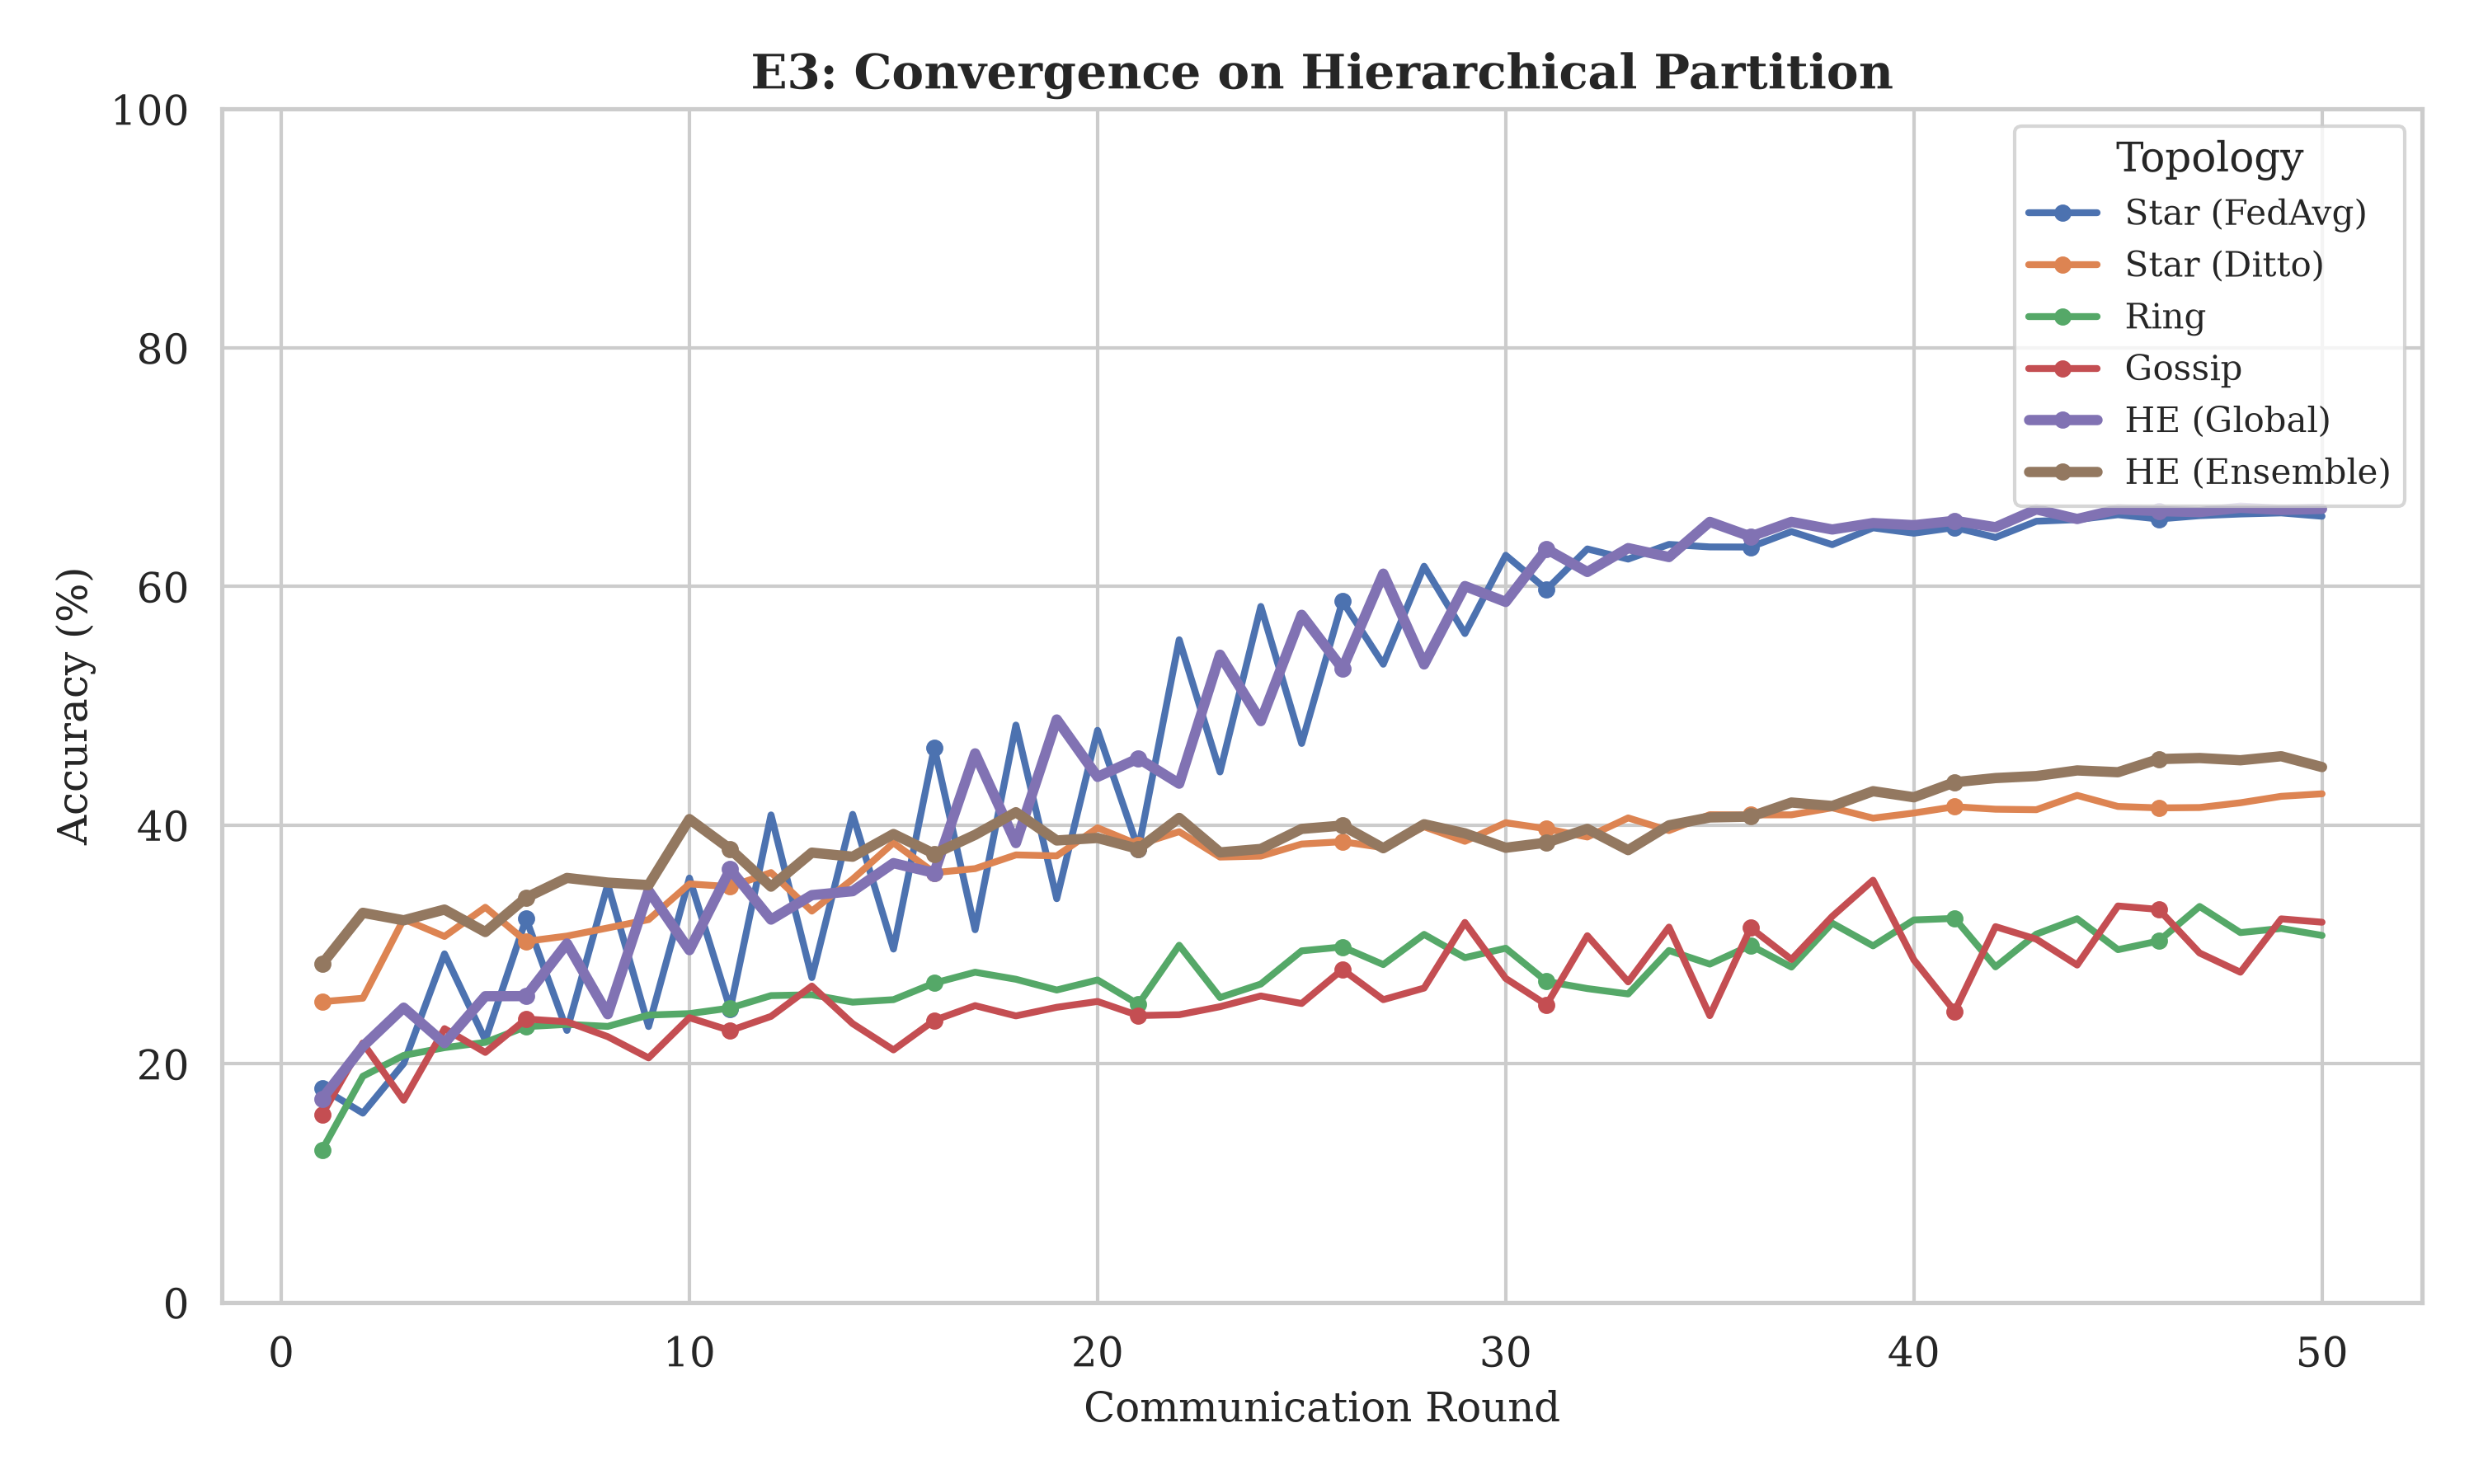
\includegraphics[width=0.75\textwidth]{partA_E3_hierarchical_accuracy.png}
    \caption{Convergence trajectories on Bilevel Hierarchical Partition over 50 communication rounds.}
    \label{fig:e3}
\end{figure}

\begin{table}[H]
    \centering
    \begin{tabular}{lc}
        \toprule
        \textbf{Topology} & \textbf{Final Accuracy (\%)} \\
        \midrule
        HE (Global) & 66.50 \\
        Star (FedAvg) — global & 65.88 \\
        HE (Ensemble) — personalized & 44.86 \\
        Star (Ditto) — personalized & 42.62 \\
        Gossip ($k=3$) & 31.86 \\
        Ring & 30.75 \\
        \bottomrule
    \end{tabular}
    \caption{Final Accuracy (Round 50) — Bilevel Hierarchical Partition}
\end{table}

Under the bilevel hierarchical partition, all models experience lower test accuracy due to extreme inter-cluster skew. Notably, HE Global (66.50\%) exceeds HE Ensemble (44.86\%), inverting the performance relationship observed in the standard non-IID setting. When clusters specialize heavily in disjoint subsets of classes, localized personalized heads overfit to cluster-specific distributions, whereas global models benefit from integrating representations across disparate clusters.

\subsection{Byzantine Robustness on Standard Non-IID Partition}
\begin{figure}[H]
    \centering
    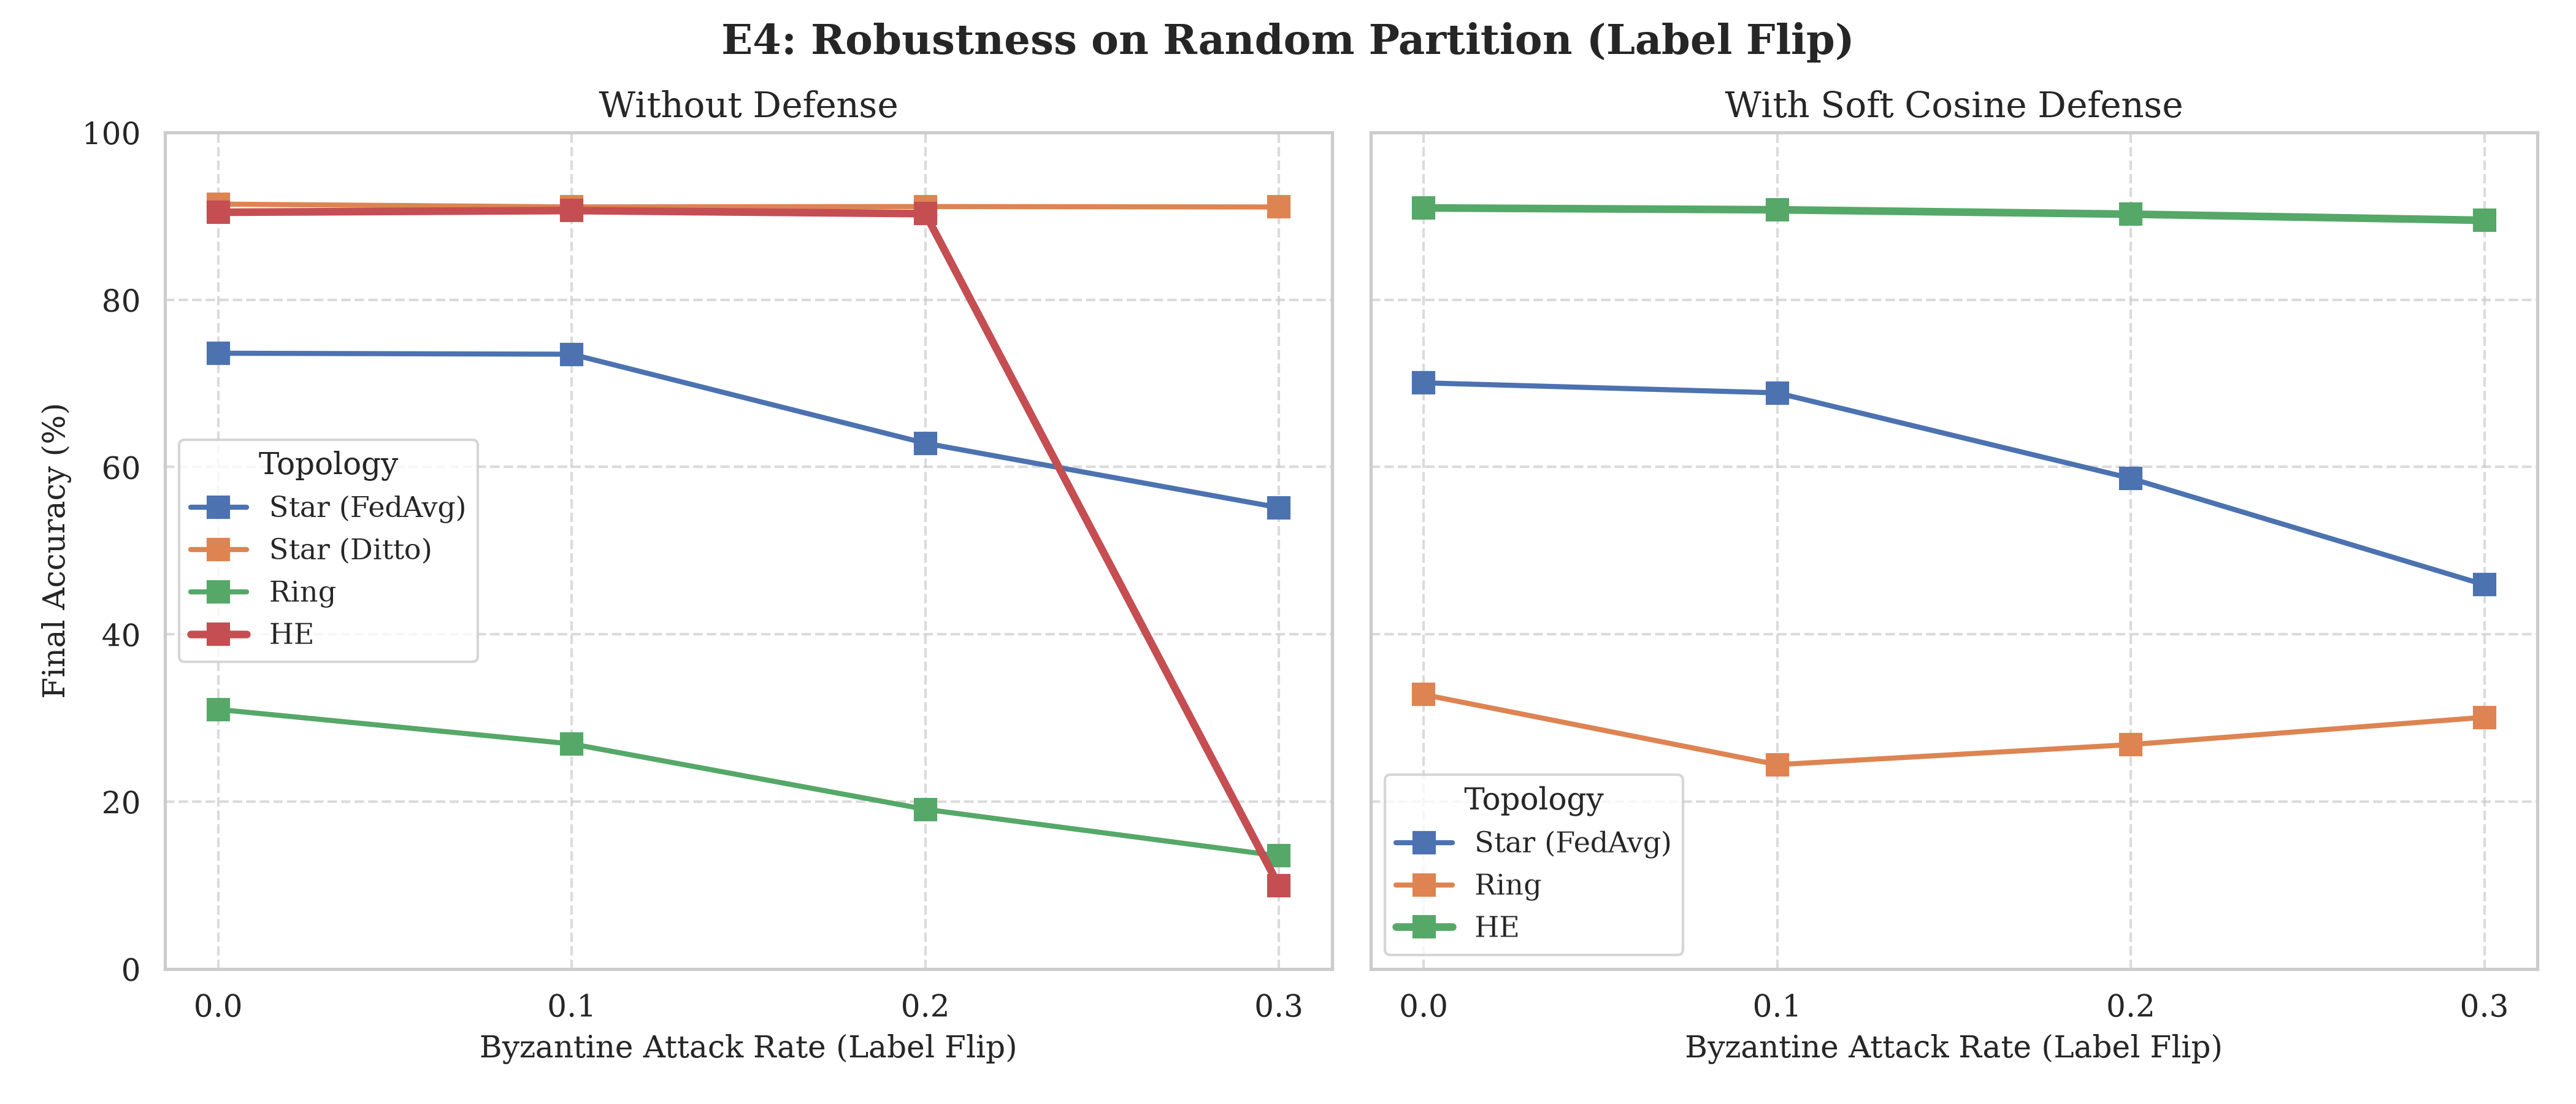
\includegraphics[width=0.88\textwidth]{partB_E4_robustness.png}
    \caption{Byzantine robustness comparison on Random Partition under label flipping (Left: Undefended, Right: Soft Cosine Defense).}
    \label{fig:e4}
\end{figure}

\begin{table}[H]
    \centering
    \begin{tabular}{llccccc}
        \toprule
        \textbf{Topology} & \textbf{Defense} & \textbf{q=0.0} & \textbf{q=0.1} & \textbf{q=0.2} & \textbf{q=0.3} & \textbf{$\Delta$(0$\rightarrow$0.3)} \\
        \midrule
        Star (Ditto) & None & 91.44 & 91.10 & 91.14 & 91.09 & -0.35 \\
        HE & None & 90.46 & 90.67 & 90.29 & 9.95 & -80.51 \\
        Star (FedAvg)& None & 73.61 & 73.49 & 62.85 & 55.15 & -18.46 \\
        Ring & None & 31.02 & 26.90 & 19.08 & 13.51 & -17.51 \\
        \midrule
        HE & Full Defense & 90.98 & 90.76 & 90.23 & 89.50 & -1.48 \\
        Star (FedAvg)& Full Defense & 70.07 & 68.87 & 58.65 & 45.93 & -24.14 \\
        Ring & Full Defense & 32.80 & 24.42 & 26.82 & 30.08 & -2.72 \\
        \bottomrule
    \end{tabular}
    \caption{Final Accuracy (\%) across Attack Fractions ($q$) — Random Partition}
\end{table}

In the absence of defense mechanisms, the HE topology exhibits severe vulnerability once the adversary fraction reaches $q=0.3$, where accuracy declines from 90.29\% ($q=0.2$) to 9.95\%. However, integrating Soft Cosine Full Defense prevents this degradation, preserving an accuracy of 89.50\% at $q=0.3$ ($\Delta = -1.48\%$). Ditto exhibits inherent resilience to label flipping via its local proximal loss without explicit filtering, though it incurs additional memory overhead for maintaining dual models.

\subsection{Byzantine Robustness on Bilevel Hierarchical Partition}
\begin{figure}[H]
    \centering
    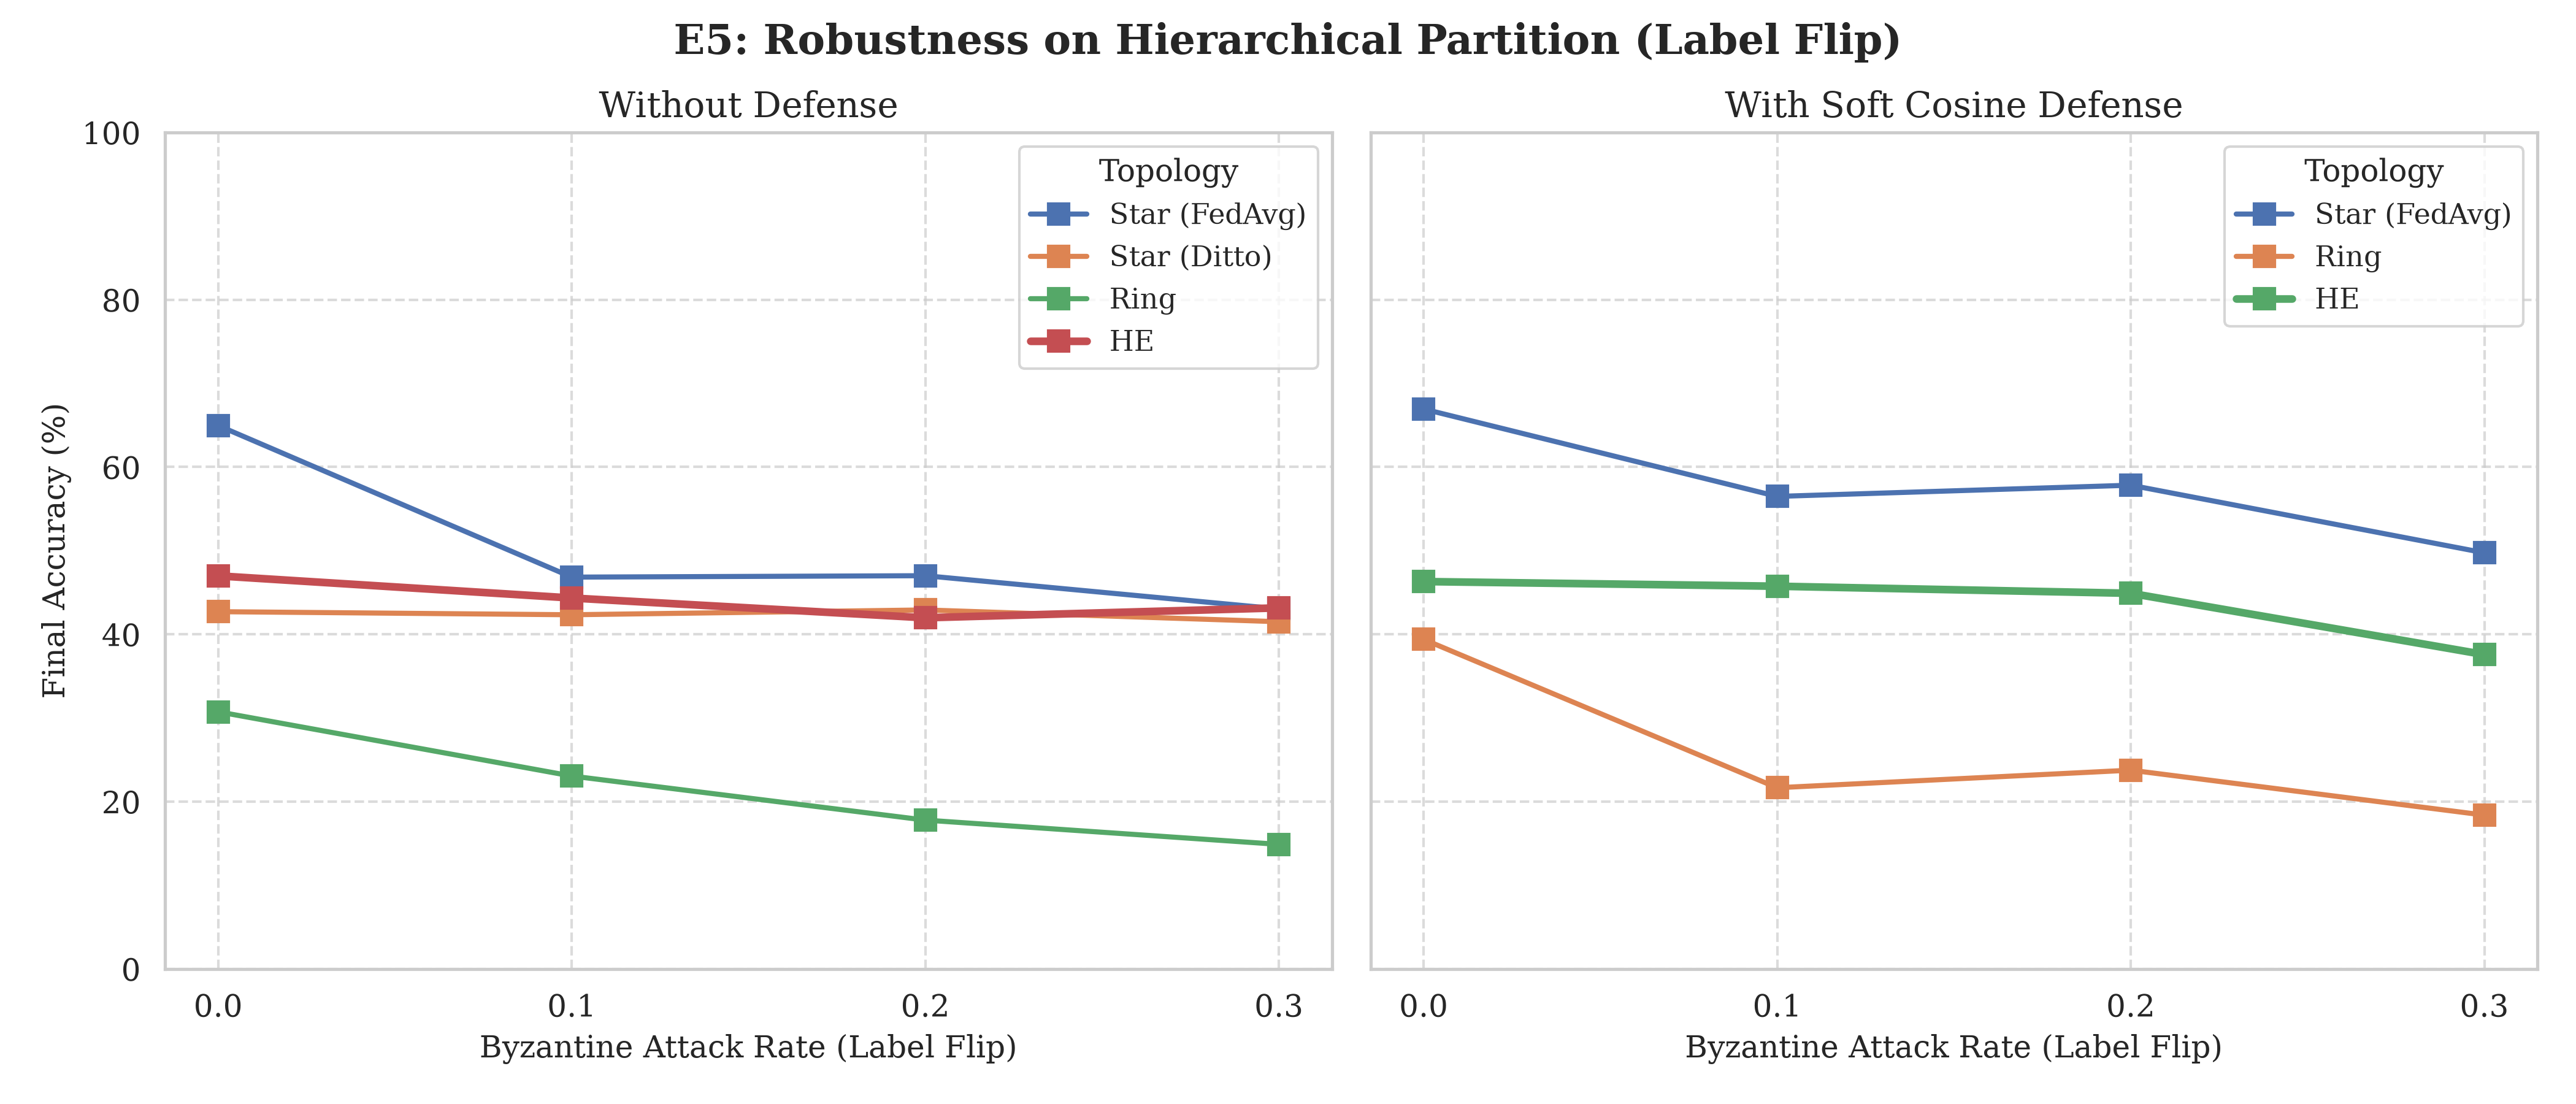
\includegraphics[width=0.88\textwidth]{partB_E5_robustness.png}
    \caption{Byzantine robustness comparison on Hierarchical Partition under label flipping (Left: Undefended, Right: Soft Cosine Defense).}
    \label{fig:e5}
\end{figure}

\begin{table}[H]
    \centering
    \begin{tabular}{llccccc}
        \toprule
        \textbf{Topology} & \textbf{Defense} & \textbf{q=0.0} & \textbf{q=0.1} & \textbf{q=0.2} & \textbf{q=0.3} & \textbf{$\Delta$(0$\rightarrow$0.3)} \\
        \midrule
        Star (FedAvg)& None & 64.96 & 46.84 & 47.01 & 43.04 & -21.92 \\
        HE & None & 46.99 & 44.34 & 41.98 & 43.16 & -3.83 \\
        Star (Ditto) & None & 42.71 & 42.34 & 42.92 & 41.51 & -1.20 \\
        Ring & None & 30.74 & 23.06 & 17.79 & 14.89 & -15.85 \\
        \midrule
        Star (FedAvg)& Full Defense & 66.94 & 56.49 & 57.83 & 49.75 & -17.19 \\
        HE & Full Defense & 46.31 & 45.75 & 44.91 & 37.58 & -8.73 \\
        Ring & Full Defense & 39.40 & 21.66 & 23.76 & 18.39 & -21.01 \\
        \bottomrule
    \end{tabular}
    \caption{Final Accuracy (\%) across Attack Fractions ($q$) — Bilevel Hierarchical Partition}
\end{table}

Under the hierarchical partition, undefended HE exhibits smaller absolute variation under attack ($\Delta = -3.83\%$), as clustered aggregation partially localizes adversarial updates. However, Star (FedAvg) with Full Defense maintains the highest absolute test accuracy (49.75\% at $q=0.3$).

\subsection{Cross-Experiment Synthesis}
\begin{table}[H]
    \centering
    \begin{tabular}{lll}
        \toprule
        \textbf{Scenario} & \textbf{Best Topology (No Defense)} & \textbf{Best Topology (With Defense)} \\
        \midrule
        Random Partition, $q=0.0$ & Ditto (91.35\%) & — \\
        Random Partition, $q=0.3$ & Ditto (91.09\%) & HE Full (89.50\%) \\
        Hierarchical Partition, $q=0.0$ & HE Global (66.50\%) & — \\
        Hierarchical Partition, $q=0.3$ & HE No Defense (43.16\%) & Star Full (49.75\%) \\
        \bottomrule
    \end{tabular}
    \caption{Summary of best-performing configurations across evaluated scenarios.}
\end{table}

The empirical evaluation demonstrates that the efficacy of Byzantine defenses is tightly coupled with network topology and data partition geometry. Multi-tier filtering in HE provides strong protection under standard non-IID conditions. Conversely, under pronounced hierarchical clustering, cosine disparity arising from benign data heterogeneity can overlap with adversarial perturbations, reducing the relative separation margin of trust scoring.

\FloatBarrier

\section{Conclusion}
This study evaluated the interplay between network topologies, data partitioning strategies, and Byzantine defense mechanisms in federated learning. Results indicate that the Hierarchical Ensemble topology combined with Soft Cosine Rejection provides robust defense against label-flipping attacks on standard non-IID partitions. However, extreme inter-cluster data heterogeneity poses distinct challenges to distance- and angle-based aggregators. Future research will investigate defense-aware clustering techniques and evaluate performance on larger-scale datasets such as CIFAR-100.

\section{Acknowledgements}
I would like to thank Dr. Leandro Soriano Marcolino for his valuable guidance and mentorship throughout this project. Special thanks to my research peers for designing the underlying HE model architecture. Computational experiments were conducted using Kaggle GPU resources.

\begin{thebibliography}{9}

\bibitem{mcmahan2017}
McMahan, B., Moore, E., Ramage, D., Hampson, S., \& y Arcas, B. A. (2017). 
Communication-efficient learning of deep networks from decentralized data. 
In \textit{Artificial intelligence and statistics} (pp. 1273-1282). PMLR.

\bibitem{li2021}
Li, T., Hu, S., Beirami, A., \& Smith, V. (2021). 
Ditto: Fair and robust federated learning through personalization. 
In \textit{International Conference on Machine Learning} (pp. 6357-6368). PMLR.

\bibitem{blanchard2017}
Blanchard, P., El Mhamdi, E. M., Guerraoui, R., \& Stainer, J. (2017). 
Machine learning with adversaries: Byzantine tolerant gradient descent. 
\textit{Advances in neural information processing systems}, 30.

\bibitem{yin2018}
Yin, D., Chen, Y., Kannan, R., \& Bartlett, P. (2018). 
Byzantine-robust distributed learning: Towards optimal statistical rates. 
\textit{International Conference on Machine Learning} (pp. 5650-5659). PMLR.

\bibitem{fung2020}
Fung, C., Yoon, C. J., \& Beschastnikh, I. (2020). 
Mitigating sybils in federated learning poisoning. 
\textit{arXiv preprint arXiv:1808.04866}.

\bibitem{sun2019}
Sun, Z., Kairouz, P., Suresh, A. T., \& McMahan, H. B. (2019). 
Can you really backdoor federated learning? 
\textit{arXiv preprint arXiv:1911.07963}.

\bibitem{hsu2019}
Hsu, T. M. H., Qi, H., \& Brown, M. (2019). 
Measuring the effects of non-identical data distribution for federated visual classification. 
\textit{arXiv preprint arXiv:1909.06335}.

\bibitem{liu2020}
Liu, L., Zhang, J., Song, S., \& Letaief, K. B. (2020). 
Client-edge-cloud hierarchical federated learning. 
\textit{IEEE International Conference on Communications (ICC)}.

\bibitem{karimireddy2020}
Karimireddy, S. P., Kale, S., Mohri, M., Reddi, S., Stich, S., \& Suresh, A. T. (2020). 
Scaffold: Stochastic controlled averaging for federated learning. 
\textit{International Conference on Machine Learning} (pp. 5132-5143). PMLR.

\bibitem{zhao2018}
Zhao, Y., Li, M., Lai, L., Suda, N., Civin, D., \& Chandra, V. (2018). 
Federated learning with non-iid data. 
\textit{arXiv preprint arXiv:1806.00582}.

\end{thebibliography}

\end{document}
